% --------------------------------------------------------------
% This is all preamble stuff that you don't have to worry about.
% Head down to where it says "Start here"
% --------------------------------------------------------------
 
\documentclass[12pt]{article}
 
\usepackage[margin=1in]{geometry} 
\usepackage{amsmath,amsthm,amssymb}
\usepackage{hyperref}
\hypersetup{
    colorlinks,
    citecolor=black,
    filecolor=black,
    linkcolor=black,
    urlcolor=blue
}
\usepackage{graphicx}
\newcommand{\code}{\texttt}
\begin{document}
\title{Write-and-Do-Mini-Assignment\#2: Error Messages in Clang, GCC and LLVM}
\author{Sagar Jain\\CS17BTECH11034}
\maketitle
\section*{Error Handling in Clang/LLVM}
\subsubsection*{Programmatic Errors}
The observations on error messages have been made from \href{http://llvm.org/docs/ProgrammersManual.html}{here}.
In LLVM all the errors are classified into two types; \textit{programmatic} and \textit{recoverable}. Assertions are used heavily in the llvm-project. An assertion can be made to check if any code invariant or condition is being broken.\\
For example:\\
In \code{clang/lib/Analysis/CallGraph.cpp} we can find the following:\\
\hspace*{5ex} \code{assert(*CI != Root \&\& "No one can call the root node.")}
\\ We know that in a cfg there can be no calls to the root node, this assert is placed in the code to ensure this condition and also holds a message so that the user can know why the program has stopped execution.
\subsubsection*{Recoverable Errors}
Recoverable errors are mostly the errors which occur because of reasons other than mistakes in the source code. These errors should be reported to the user as well. Reported errors are handled using the error scheme provided by LLVM. The error class can be used for any user defined errors and we can also specify information regarding the error in it. Template functions like \code{make\_error} are provided to construct failure values for the error class created by us which inherit from \code{ErrorInfo}.
\subsubsection*{•}
The following files define the most important error handling apis and methods in LLVM:
\begin{enumerate}
\item \texttt{ErrorHandling.h}: This file defines an API used to indicate fatal error conditions.
\item \texttt{Error.h}: This file defines an API used to report recoverable errors.
\item \texttt{ErrorOr.h}: Provides ErrorOr$\langle$T$\rangle$ smart pointer.\\
This is a very important pointer. This template pointer either has the value of an operation of type T or an error, on error we not only have the error code but also other user information which further helps in debugging.
\item \texttt{Errno.h}: This file declares some portable and convenient functions to deal with errno. 
\end{enumerate}
\section*{Error Handling in GCC}
GCC reports two kinds of debugging information to users: \textit{warnings} and \textit{errors}.\\
For C the, file where most of the error/warning methods are defined is \texttt{gcc/diagnostic-core.h}. Some most important functions used by gcc to report errors are:
\begin{itemize}
\item error\_at
\item warning\_at
\item fatal\_error
\item pedwarn (pedantic warnings), etc.
\end{itemize}
These functions are not called directly but through local functions defined at the level any one compiler component. Almost all the error reporting follows the same pattern where the error is discovered at the particular component and is sent down through a fixed set of functions to one of the functions mentioned above.These functions usually take arguments of the type location\_t.\\\\ 
The following is an example of how a parser-error would make it to the user in gcc.
Observations made from source files at \href{https://github.com/gcc-mirror/gcc/tree/5fe20025f581fb0c215611434d76696161d4cbd3/gcc/c}{link} \\\\
\begin{center}
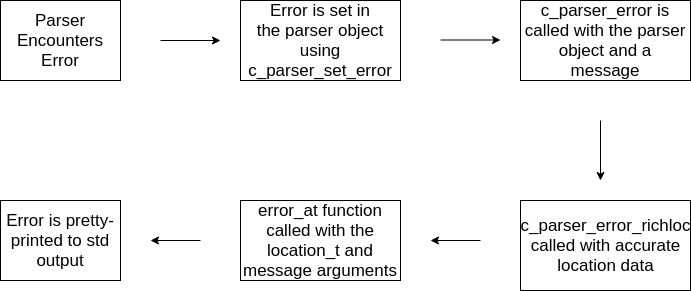
\includegraphics[scale=0.65]{gcc.png}
Used \href{https://www.draw.io}{this} for flowchart construction.
\end{center}

\end{document}